\documentclass[../main.tex]{subfiles}
\graphicspath{{\subfix{./figs/}}}

\begin{document}

\chapter{Fits}\label{appendix:a}
\section{Double Gaussian}
Explicitly, the double Gaussian fit is given by:

\begin{align}
    \frac{dN}{d\Delta\varphi} = &A_{\text{NS}} \exp{\left(\frac{-1}{2}\left(\frac{\Delta\varphi-\mu_{\text{NS}}}{\sigma_{\text{NS}}}\right)^2\right)} \\
    &+ A_{\text{AS}} \exp{\left(\frac{-1}{2}\left(\frac{\Delta\varphi-\mu_{\text{AS}}}{\sigma_{\text{AS}}}\right)^2\right)} 
\end{align}

where $\sigma$ is the standard deviation, $\mu$ is the mean, and the subscripts on the fitted parameters indicate the near- and away-side. The uncertainty in $\sigma$ is simply obtained from the fit. All double Gaussian fits are shown in Fig. \ref{fig:gaussian_fits}.

\begin{figure}
    \centering
    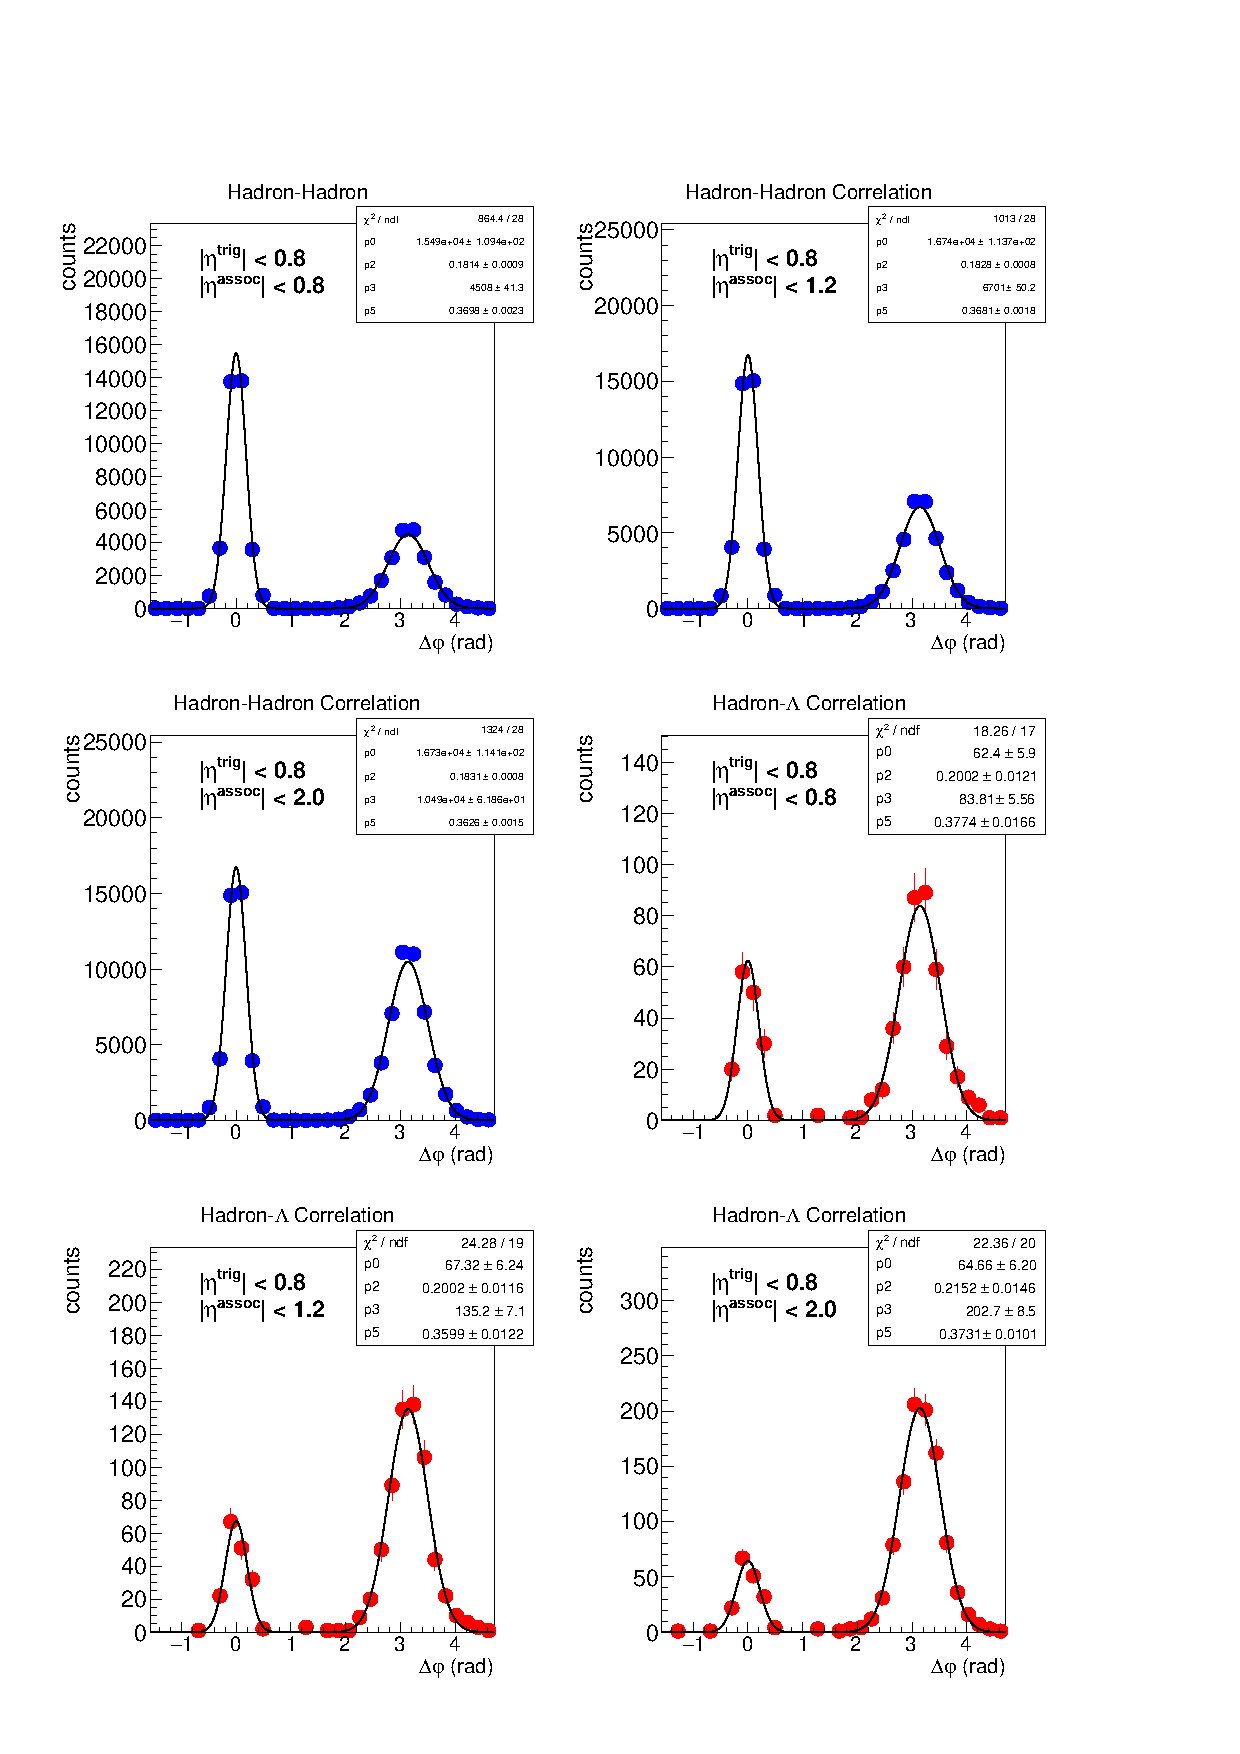
\includegraphics[scale=0.75]{appendix/figs/gaussian_fit.pdf}
    \caption{Gaussian fits for all correlations. In order, the fit parameters are $A_{\text{NS}}$, $\sigma_{\text{NS}}$, $A_{\text{AS}}$, and $\sigma_{\text{AS}}$.}
    \label{fig:gaussian_fits}
\end{figure}


\clearpage
\section{Double Generalized Gaussian}

\begin{align}
     \frac{dN}{d\Delta\varphi} =& A_{\text{NS}}\frac{\beta_{\text{NS}}}{2\alpha_{\text{NS}}\Gamma(1/\beta_{\text{NS}})}\exp{\left(-\left(\frac{|x-\mu_{\text{NS}}|}{\alpha_\text{NS}}\right)^{\beta_{\text{NS}}}\right)} \\
     &+ A_{\text{AS}}\frac{\beta_{\text{AS}}}{2\alpha_{\text{AS}}\Gamma(1/\beta_{\text{AS}})}\exp{\left(-\left(\frac{|x-\mu_{\text{AS}}|}{\alpha_\text{AS}}\right)^{\beta_{\text{AS}}}\right)}
\end{align}

where $\alpha$, $\beta$, and $\mu$ are fit parameters explained in Section \ref{sxn:fits}, and the subscripts denote whether the term fits the near- or away-side. The standard deviation from this fit is given in Eq. \ref{eq:gengaussigma}. For a given generalized Gaussian, the uncertainty in the standard deviation is given by

\begin{equation}
    s_{\sigma} = \sqrt{\left(\frac{\partial \sigma}{\partial \alpha} \sigma_\alpha\right)^2 + \left(\frac{\partial \sigma}{\partial \beta} \sigma_\beta\right)^2}
\end{equation}

where $s_\sigma$ is the uncertainty in the standard deviation, $\sigma$ is the standard deviation, and $\sigma_\alpha$ and $\sigma_\beta$ are the uncertainties in the fit parameters. All double generalized Gaussian fits are shown in Fig. \ref{fig:gen_gaussian_fits}. To explicitly write these partial derivatives, we must introduce the polygamma function of order zero, also known as the digamma function:

\begin{equation}
    \psi(x) = \frac{\Gamma'(x)}{\Gamma(x)}
\end{equation}

so that

\begin{equation}
    \frac{\partial \sigma}{\partial \alpha} = \frac{\sigma}{\alpha}
\end{equation}

\begin{equation}
    \frac{\partial \sigma}{\partial \beta} = \frac{\sigma}{2 \beta^2} (\psi(1/\beta) - 3 \psi(3/\beta))
\end{equation}


\begin{figure}
    \centering
    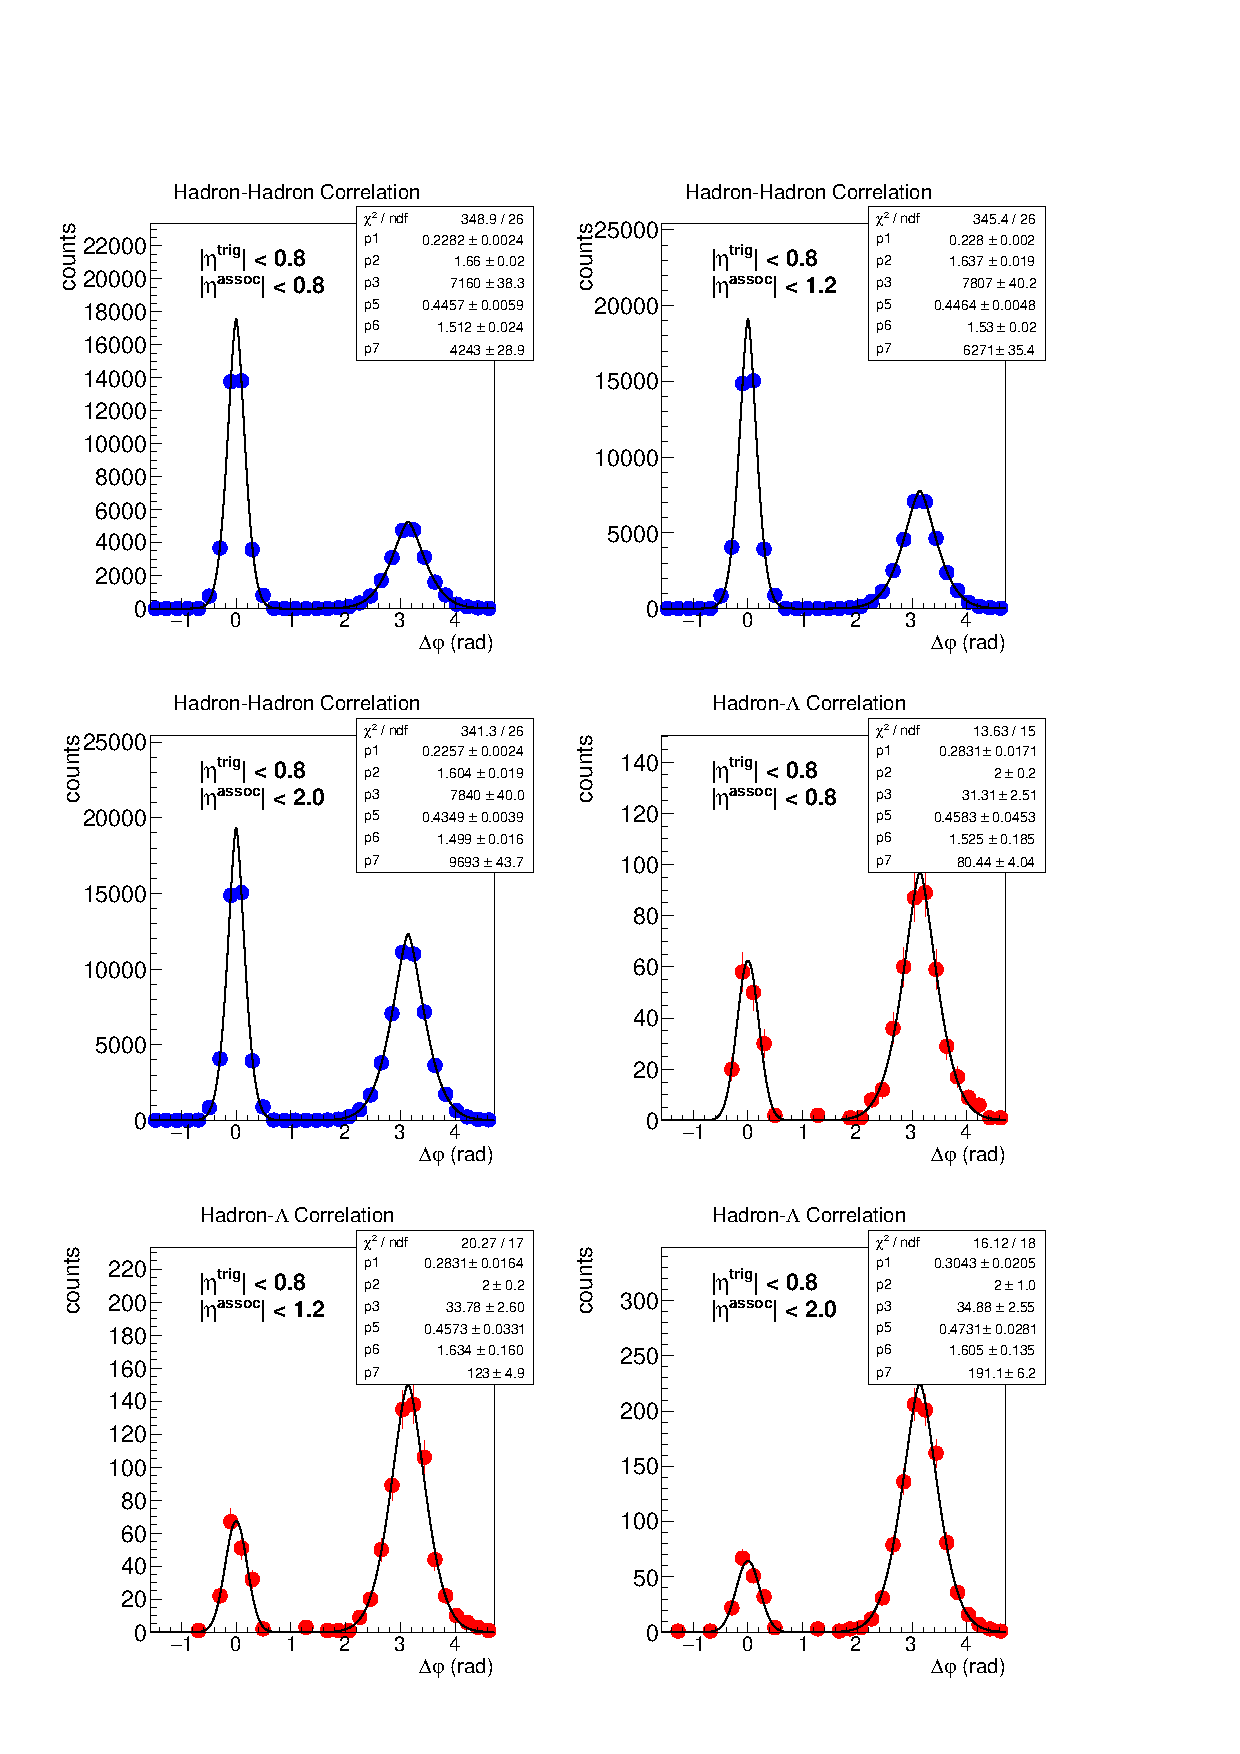
\includegraphics[scale=0.75]{appendix/figs/gen_gaussian_fit.pdf}
    \caption{Generalized Gaussian fits for all correlations. In order, the fit parameters are $\alpha_{\text{NS}}$, $\beta_{\text{NS}}$, $A_{\text{NS}}$, $\alpha_{\text{AS}}$, $\beta_{\text{AS}}$, $A_{\text{AS}}$.}
    \label{fig:gen_gaussian_fits}
\end{figure}


\clearpage
\section{Double Von Mises}

\begin{align}
    \frac{dN}{d\Delta\varphi} =& A_{\text{NS}}\frac{\exp{(\kappa_{\text{NS}} \cos{(x-\mu_{\text{NS}})})}}{2\pi I_0(\kappa_\text{NS})} \\
    &+ A_{\text{AS}} \frac{\exp{(\kappa_{\text{AS}} \cos{(x-\mu_{\text{AS}})})}}{2\pi I_0(\kappa_\text{AS})}
\end{align}

where $\kappa$ and $\mu$ are fit parameters explained in Section \ref{sxn:fits}. These fits are shown in Fig. \ref{fig:mises_fits}. For the Von Mises, the uncertainty in the standard deviation is simply:

\begin{equation}
    s_\sigma = \frac{\partial \sigma}{\partial \kappa} \sigma_\kappa = \frac{1}{\sigma} \left(\frac{I_1}{I_0} - \frac{I_0}{I_1} + \frac{1}{\kappa}\right) \sigma_\kappa
\end{equation}

\begin{figure}
    \centering
    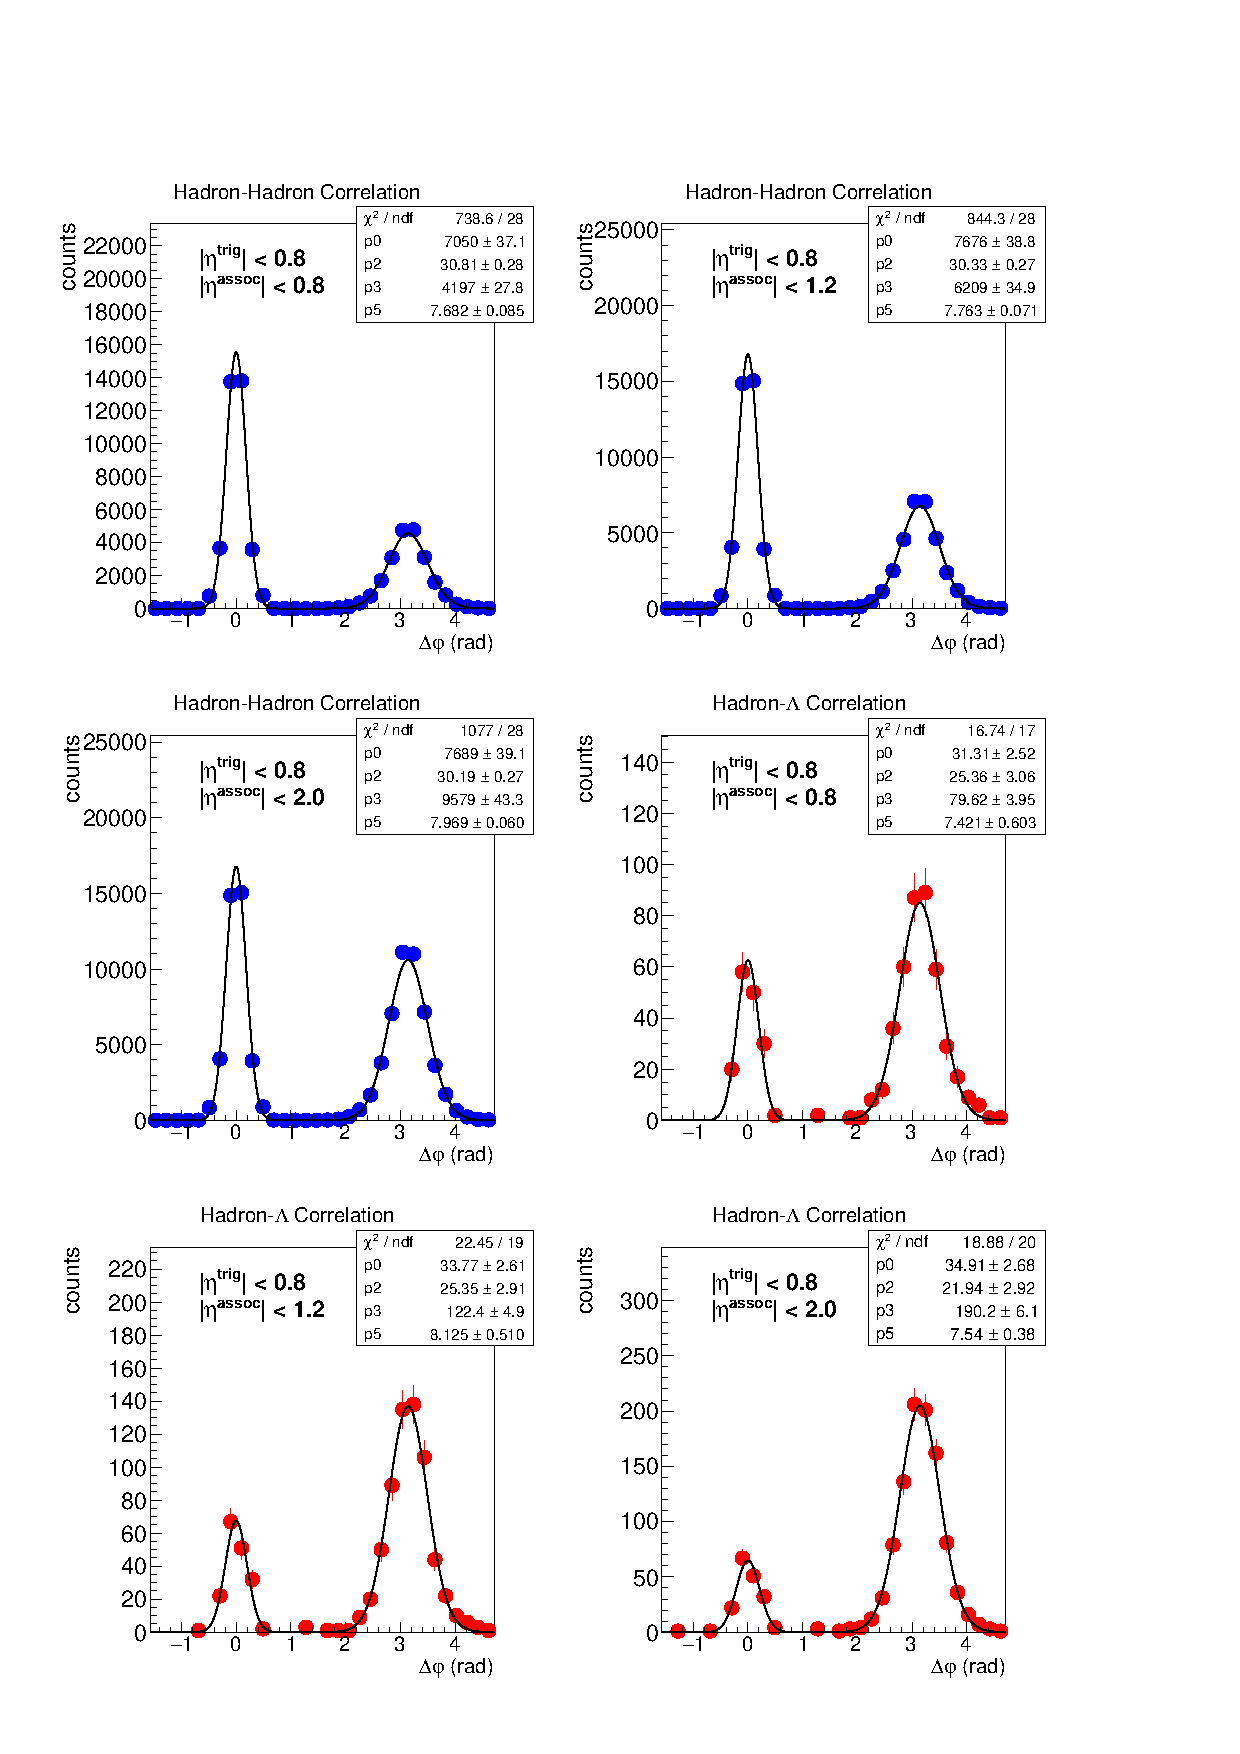
\includegraphics[scale=0.75]{appendix/figs/mises_fit.pdf}
    \caption{Von Mises fits for all correlations. In order, the fit parameters are $A_{\text{NS}}$, $\kappa_{\text{NS}}$, $A_{\text{AS}}$, and $\kappa_{\text{AS}}$.}
    \label{fig:mises_fits}
\end{figure}

\clearpage
\chapter{Dense Yield Ratios} \label{appendix:b}
For thoroughness, we also include yield ratios for more $\eta$ cuts. These are then fitted to a simple linear fit, and we find the slopes agree with 0, indicating no measurable effects from acceptance. 

\begin{figure}[h]
    \centering
    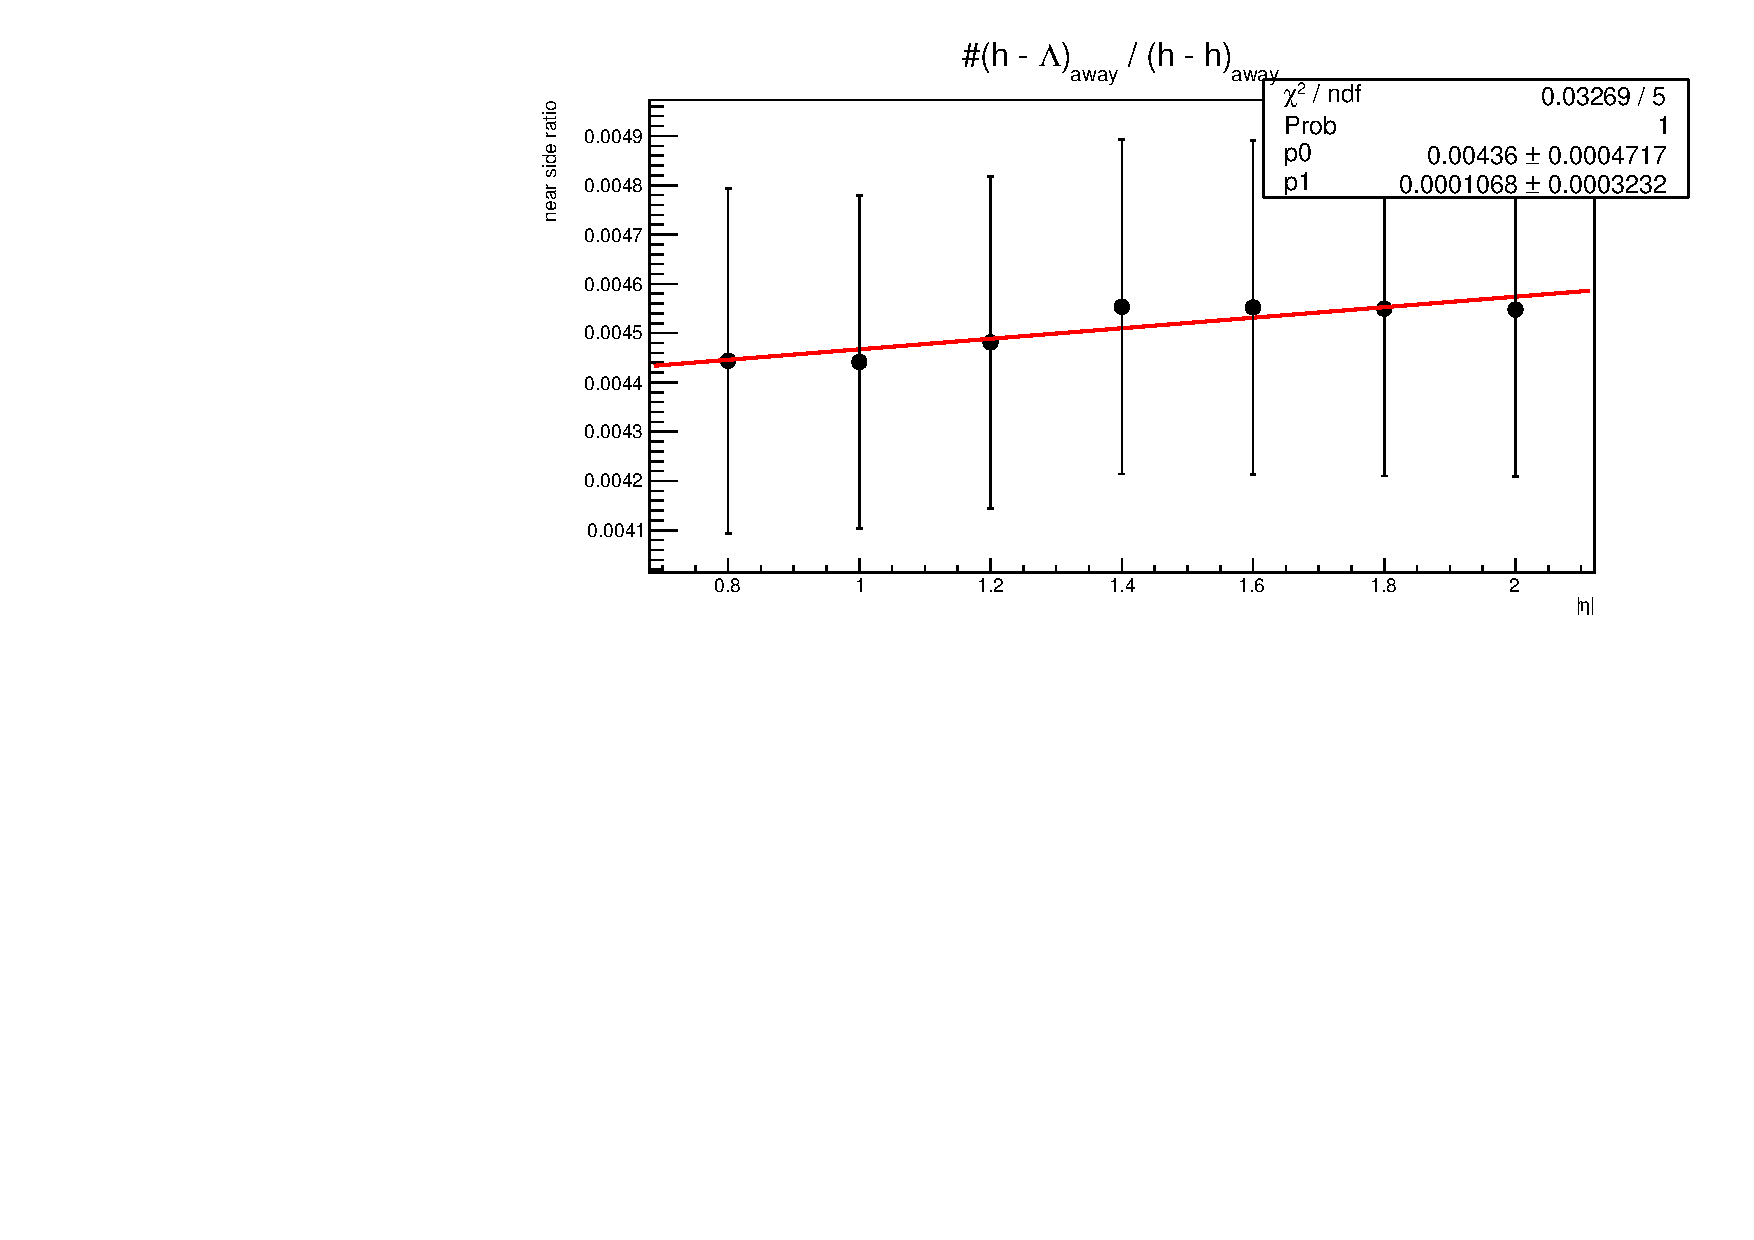
\includegraphics[scale=0.45]{appendix/figs/dense_yield_near.pdf}
    \caption{Yield ratios for the near-side across many $\eta$ cuts on the associated. The slope agrees with zero. }
    \label{fig:enter-label}
\end{figure}

\begin{figure}[h]
    \centering
    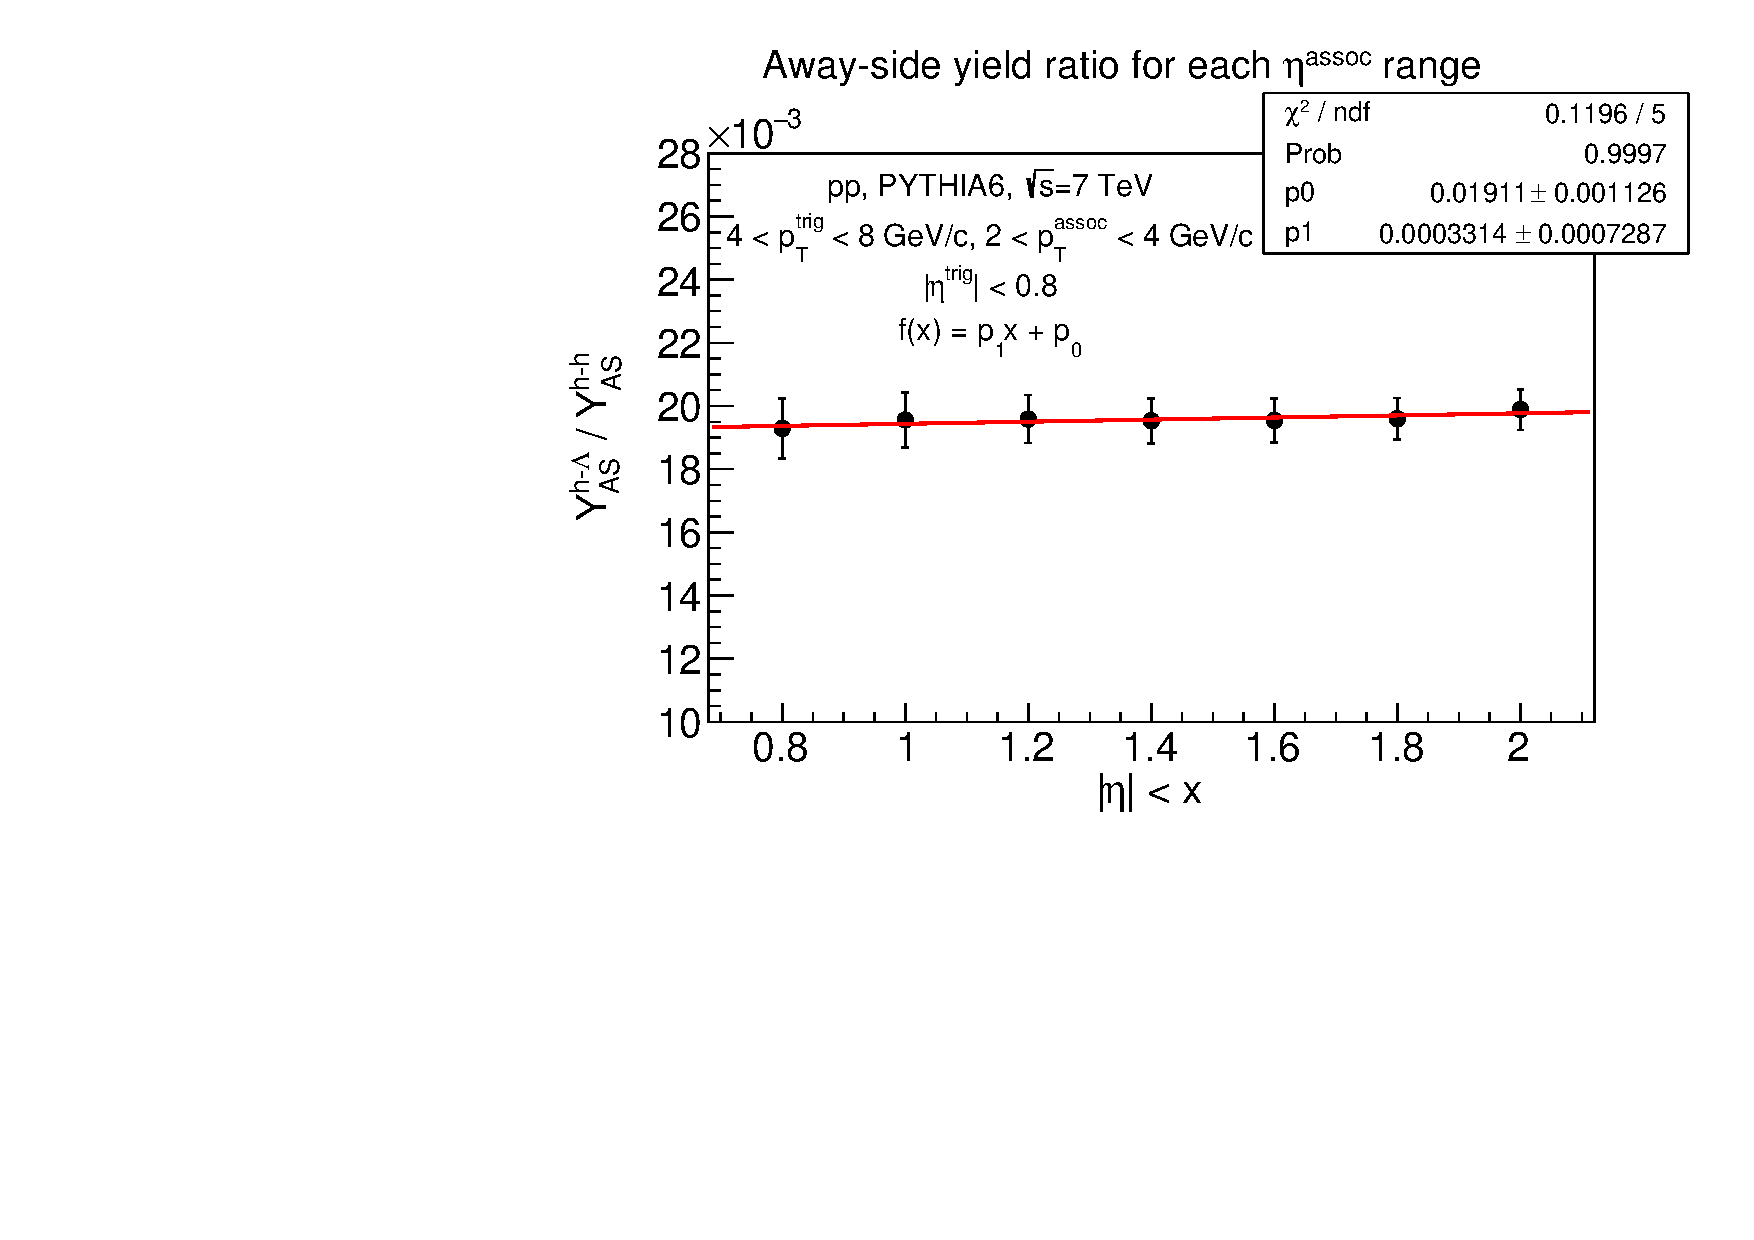
\includegraphics[scale=0.45]{appendix/figs/dense_yield_away.pdf}
    \caption{Yield ratios for the away-side across many $\eta$ cuts on the associated. The slope agrees with zero. }
    \label{fig:enter-label}
\end{figure}

\end{document}